\documentclass[tikz,border=8pt]{standalone}
% Shared look for every TikZ diagram. Load with \input{../../tools/tikz-style.tex}
\usepackage[T1]{fontenc}
\usepackage{lmodern}
\renewcommand{\sfdefault}{lmr}  % diagrams use the same serif as the text
\usetikzlibrary{arrows.meta, positioning, shapes.geometric, calc, fit, backgrounds}
\definecolor{cblue}{HTML}{4C78A8}
\definecolor{corange}{HTML}{F58518}
\definecolor{cgreen}{HTML}{54A24B}
\definecolor{cred}{HTML}{E45756}
\definecolor{cpurple}{HTML}{B279A2}
\definecolor{cgrey}{HTML}{6B6B6B}
\tikzset{
  every picture/.style={font=\sffamily, line width=1.2pt},
  box/.style={draw=#1, fill=#1!12, rounded corners=4pt, align=center, inner sep=7pt, minimum height=1.1cm},
  box/.default=cgrey,
  arrow/.style={-{Stealth[length=3mm]}, draw=cgrey, line width=1.4pt},
  title/.style={font=\sffamily\bfseries\Large},
  note/.style={font=\sffamily\small, text=cgrey, align=center},
}
\AtBeginDocument{\hyphenpenalty=10000 \exhyphenpenalty=10000}

\begin{document}
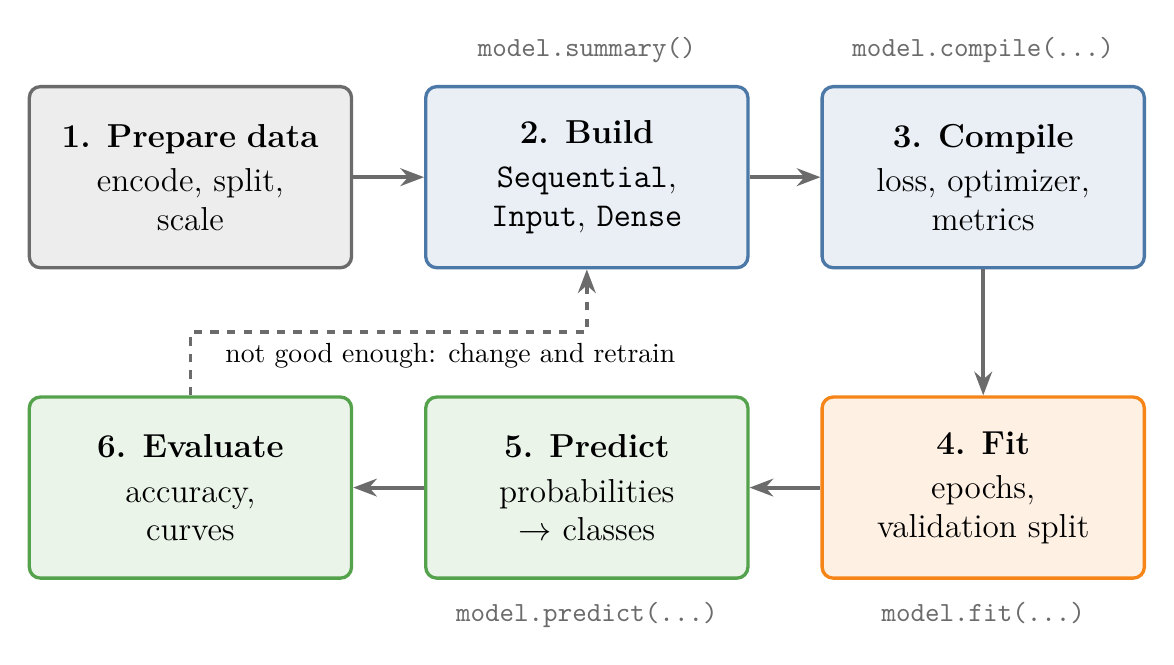
\begin{tikzpicture}[node distance=0.9cm,
  step/.style={box=#1, text width=3.6cm, minimum height=2.3cm, font=\sffamily\large},
  code/.style={font=\ttfamily\normalsize, text=cgrey}]
  \node[step=cgrey] (data) {\textbf{1. Prepare data}\\[2pt]encode, split,\\scale};
  \node[step=cblue, right=of data] (build) {\textbf{2. Build}\\[2pt]\texttt{Sequential},\\\texttt{Input}, \texttt{Dense}};
  \node[step=cblue, right=of build] (compile) {\textbf{3. Compile}\\[2pt]loss, optimizer,\\metrics};
  \node[step=corange, below=1.6cm of compile] (fit) {\textbf{4. Fit}\\[2pt]epochs,\\validation split};
  \node[step=cgreen, left=of fit] (predict) {\textbf{5. Predict}\\[2pt]probabilities\\$\rightarrow$ classes};
  \node[step=cgreen, left=of predict] (eval) {\textbf{6. Evaluate}\\[2pt]accuracy,\\curves};
  \foreach \a/\b in {data/build, build/compile, compile/fit, fit/predict, predict/eval}
    \draw[arrow] (\a) -- (\b);
  \node[code, above=0.15cm of build] {model.summary()};
  \node[code, above=0.15cm of compile] {model.compile(...)};
  \node[code, below=0.15cm of fit] {model.fit(...)};
  \node[code, below=0.15cm of predict] {model.predict(...)};
  \draw[arrow, dashed] (eval.north) -- ++(0,0.8) -| node[pos=0.03, below right, font=\sffamily\normalsize] {not good enough: change and retrain} (build.south);
\end{tikzpicture}
\end{document}
